\chapter{Navigo}
\label{ChapterNavigo}

In the previous chapters, I proposed two approaches for encouraging drivers to follow certain routes, each focusing on a different phase of the navigation task. With a focus on the trip planning phase before a driver embarks on a trip, Chapter \ref{ChapterPreTrip} describes an approach that is grounded on Self-Determination Theory. Aside from displaying the usual estimated travel time, total distance and name of major roads that will be taken, there I explored the addition of motivative information to help drivers see the societal benefit of selecting an unselfish route. Familiarity information was also added to reduce the chances of non-selection because of high novelty. All design versions showed potential in encouraging the selection of unselfish routes. And although the combined use of simple positive framing and list of road names showed universal positive utility, preference, and can increase the likelihood of unselfish selection, it has less effect in making sure that drivers will keep on choosing unselfishly for other trip scenarios. Further, the participants in the earlier study performed the route choice task without realizing their stated choices in a real driving task. In this last chapter, my goal is to find support for the effectiveness of the most preferred motivative and familiarity information, and investigate whether drivers would continue following their unselfish choice after the first instance. I ask the question of ``\textit{Can motivative and familiarity information help sustain the selection of an unselfish choice?}''

When a driver is already on a trip, Chapter \ref{ChapterConversations} describes the approach that uses two-party conversations between distinct voice agents. When a driver approaches a decision point on the road (i.e. intersections) that allows for the discovery of an alternative route, a two-party conversation will be played that presents two different driving directions. In a driving simulation study, the technique was successful in convincing drivers to consider an alternative route while still preserving their agency. It was also found that having a point of comparison allowed drivers to reflect better on their choices, possibly affecting their future choices. However, the conversational approach increased driver workload, which will require further work on the timing of conversation delivery and control on the amount of information it gives. In improving the en route approach, I ask two further questions. First, ``\textit{can two-party conversations convince drivers to switch to an unselfish route?}'' And if they do choose an unselfish route at the beginning, ``\textit{can two-party conversations encourage drivers to continue following an unselfish route?}''

\begin{figure}[h]
\centering
  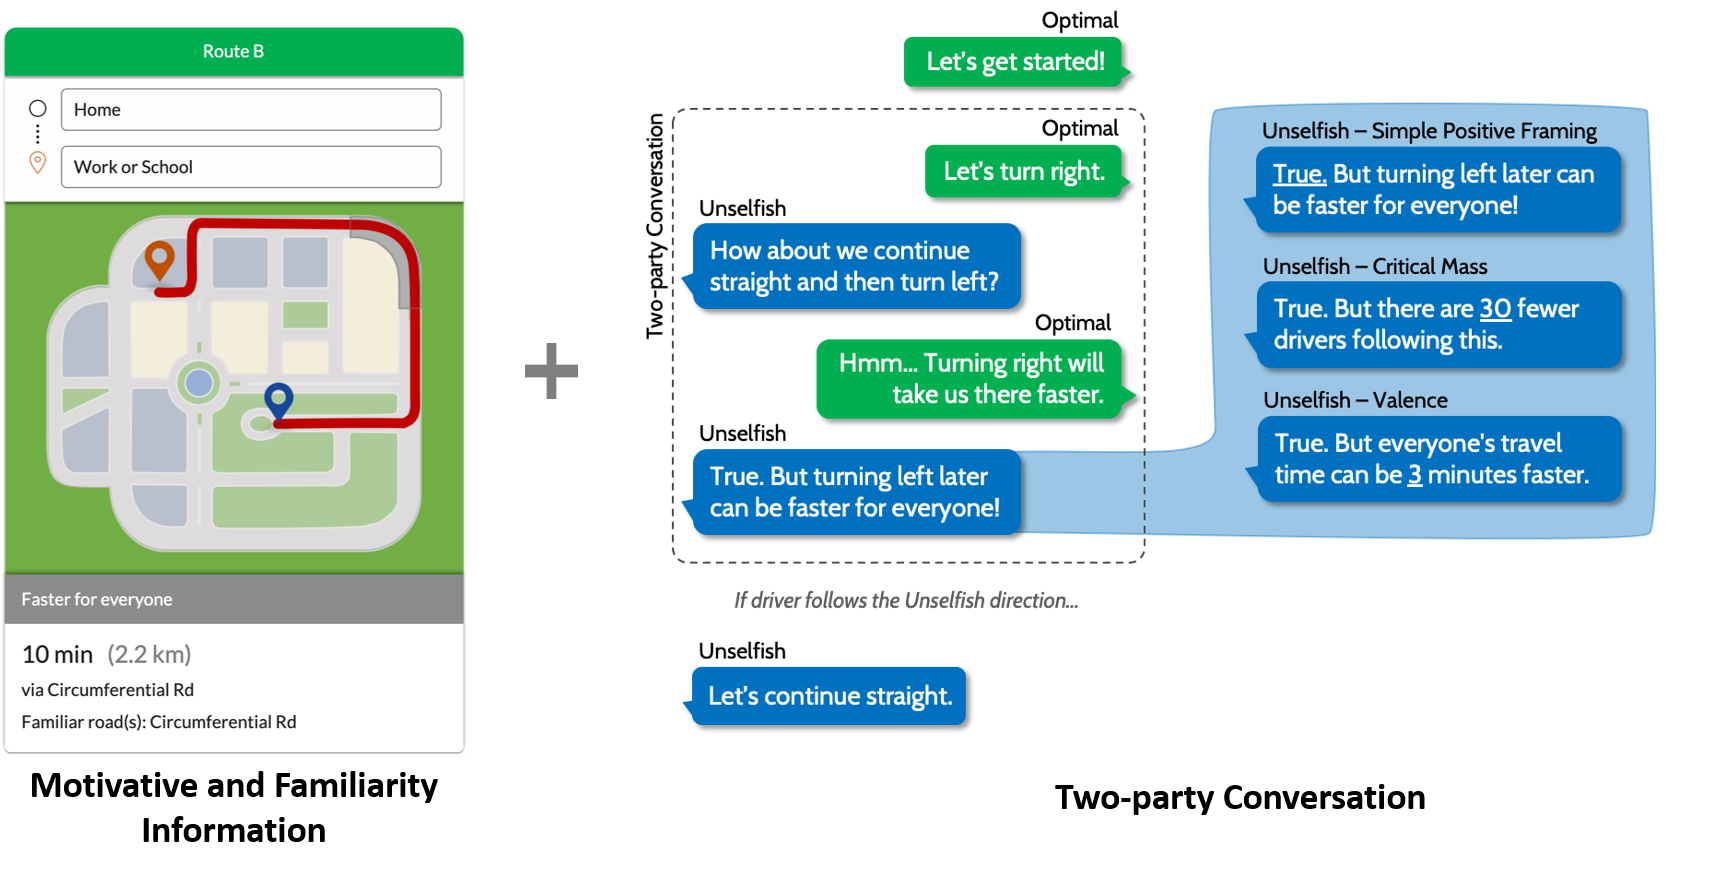
\includegraphics[scale=.5]{figures/s4-navigo.png}
  \caption{A holistic approach, Navigo refines the pre-trip (Chapter \ref{ChapterPreTrip}) and en-route techniques (Chapter \ref{ChapterConversations}), and combines them following a personality-targeted design.}~\label{fig:s4-navigo}
\end{figure}

In this chapter, I culminate my thesis by refining the two previous approaches and combining them to provide a holistic approach in encouraging drivers to choose and stick to following unselfish routes (Figure \ref{fig:s4-navigo}). This combined approach, which I call Navigo, uses personality-targeted motivative information in displaying recommended routes and in its voice guidance. When an unselfish alternative route is possible to follow, a conversation will play between two voice agents to present the next turn directions. 

\section{Holistic Approach}

Navigo's concept is close to the design approaches described in Chapters \ref{ChapterPreTrip} and \ref{ChapterConversations}. In this section, I will highlight the significant changes from the original ones. 

\begin{figure}[h]
\centering
  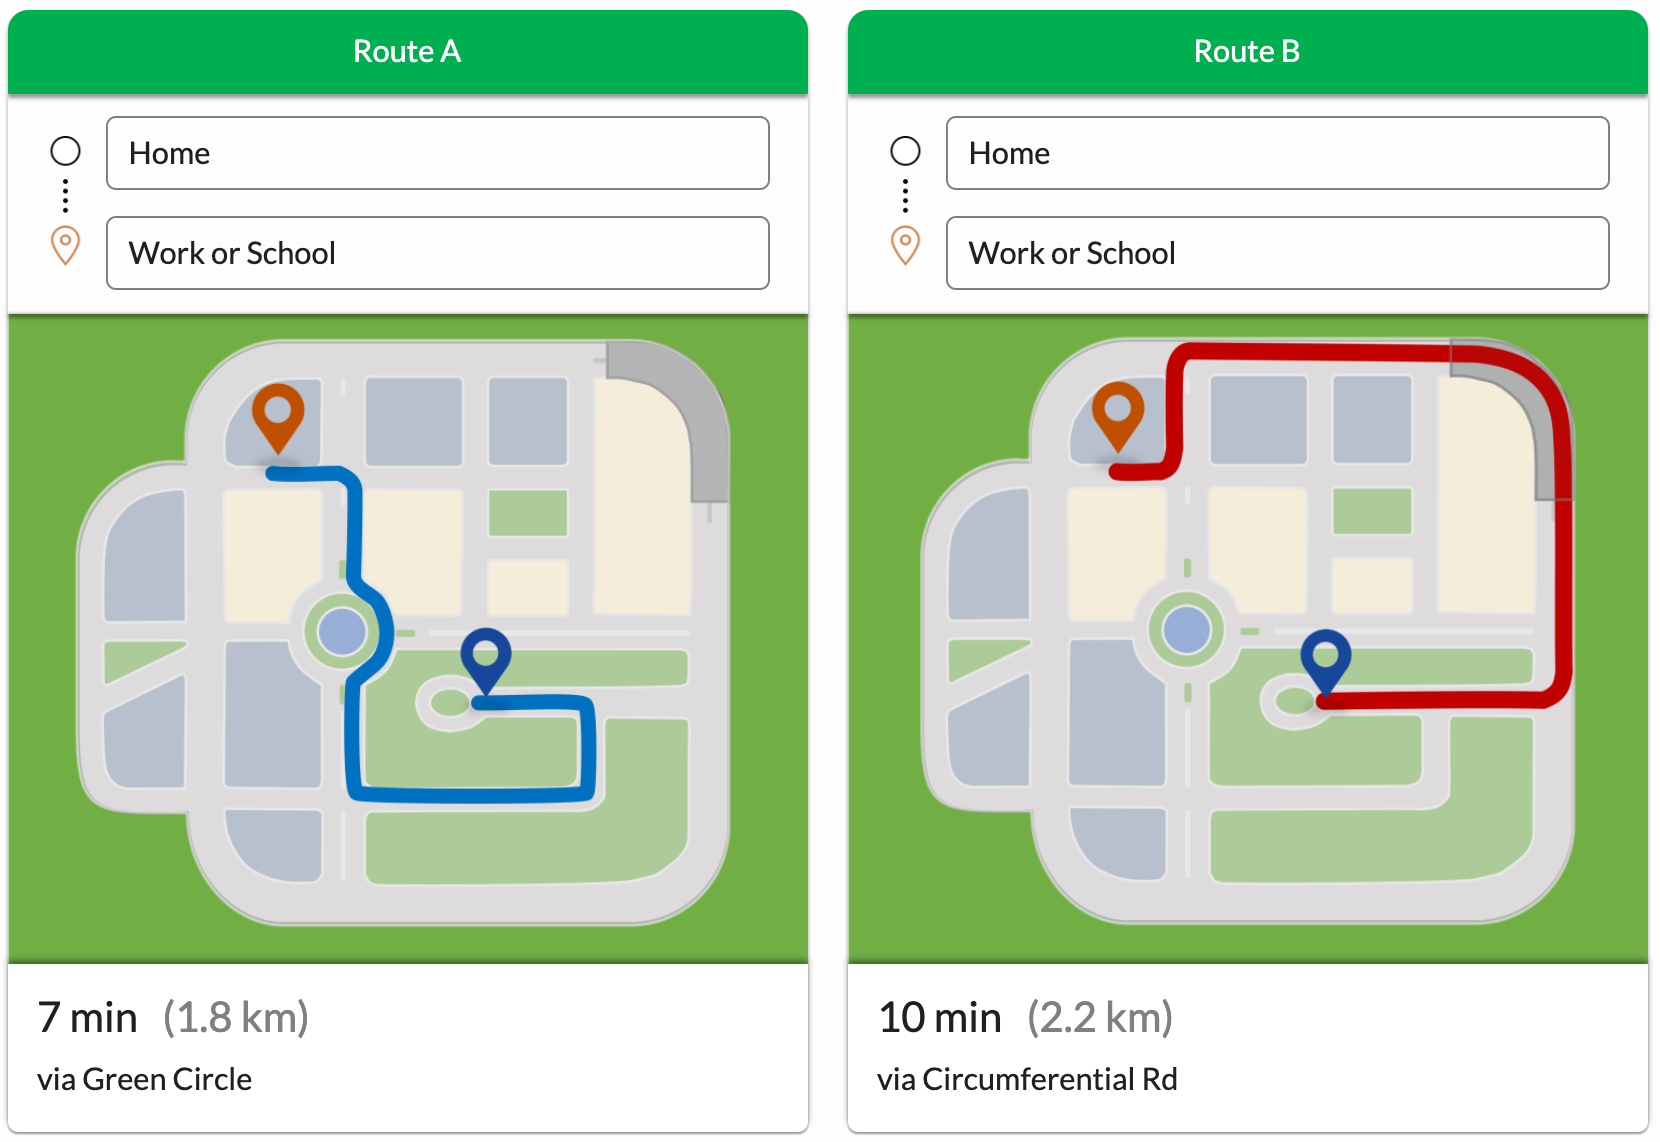
\includegraphics[scale=.4]{figures/S4-H2W-BL.png}
  \caption{The baseline version of the Navigo interface. It shows the origin and destination at the top, a map in the middle, and the trip information at the bottom.}~\label{fig:s4-bl}
\end{figure}

\subsection{Pre-Trip: Route Selection Interface}
Like in the interface described in Chapter \ref{ChapterPreTrip}, the Navigo prototype also consists of three parts (Figure \ref{fig:s4-bl}). The top shows the name of the origin and destination. The middle shows the map with an overlay of the recommended routes. The bottom area shows the trip information, which typically consists of the estimated travel time, total distance, and name of one major road included in the route. This was loosely based on the Google Maps interface. 

This interface will also have seven (7) versions that uses different combinations of the same motivative and familiarity information. The seventh design version is the baseline which shows the default set of trip information as in Figure \ref{fig:s4-bl}. 

\subsubsection{Personality-Targeted Design}

\begin{figure}[h]
\centering
  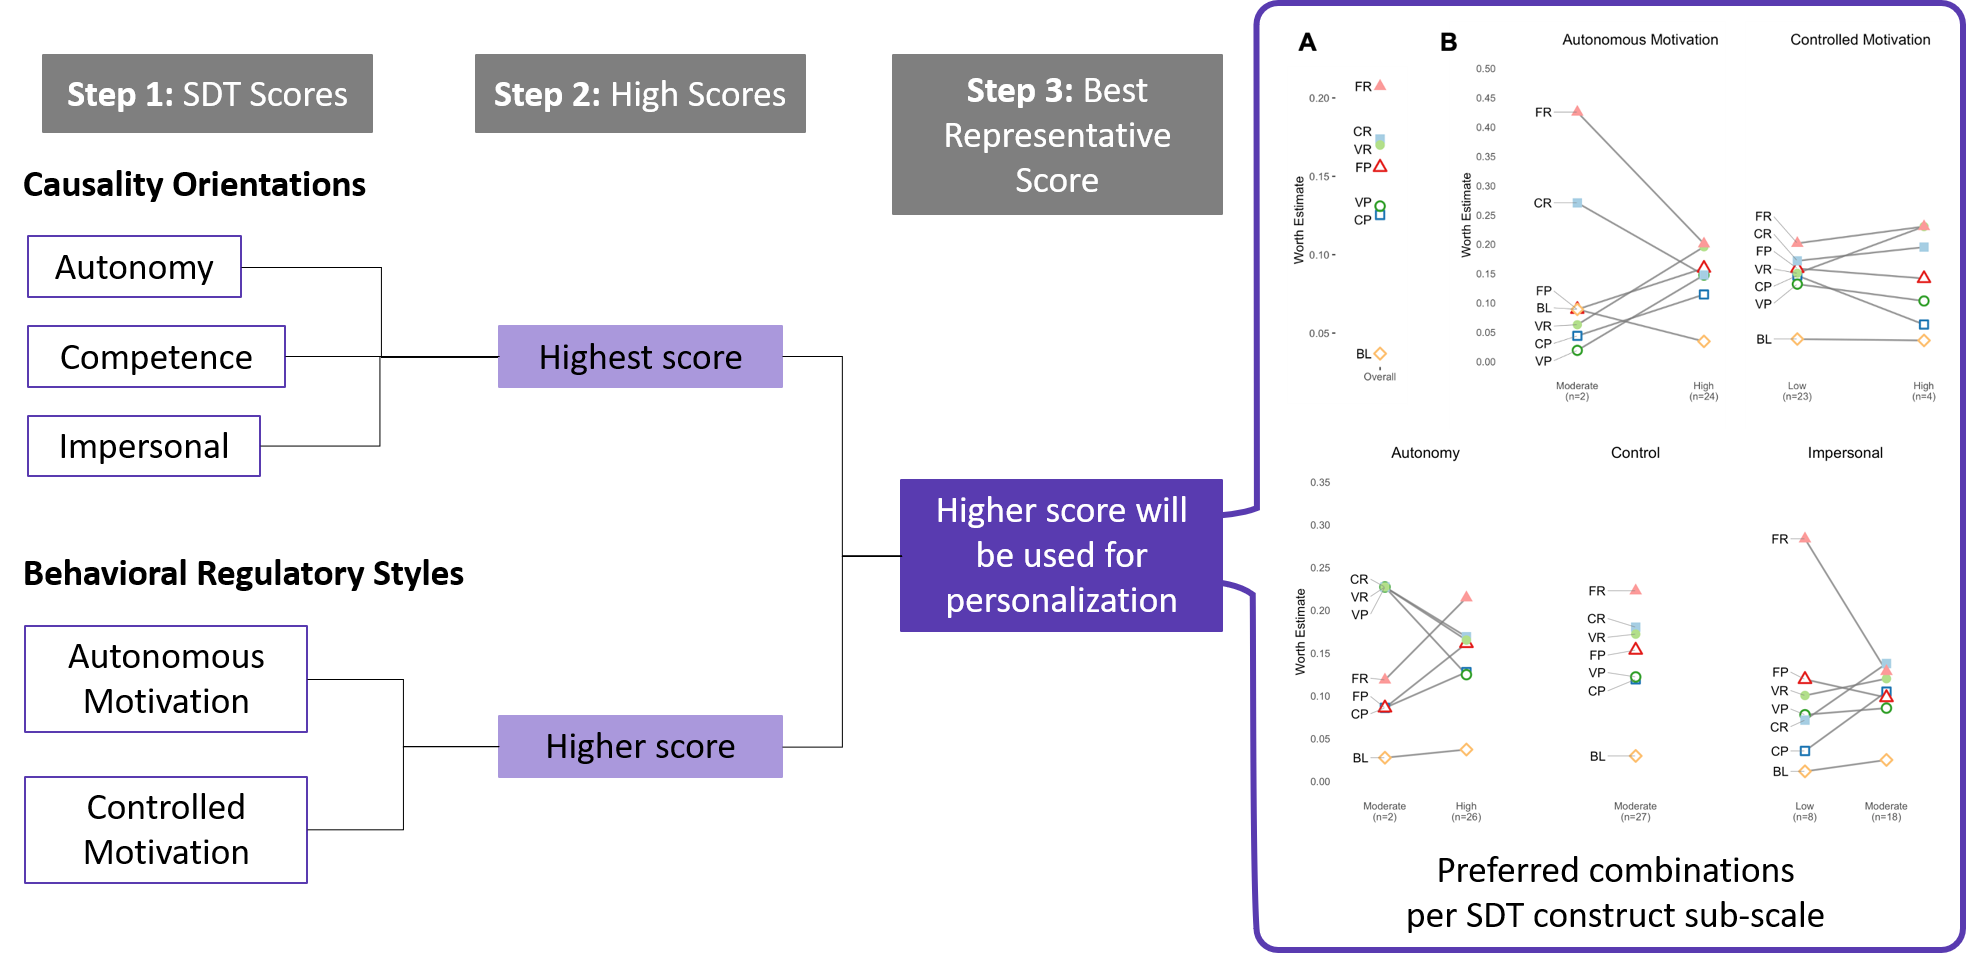
\includegraphics[scale=.45]{figures/s4-ptd.png}
  \caption{The personality-targeted design is based on the best representative score of a driver. This is an overview of the step-by-step process of selecting the the best representative scores from the causality orientation and behavioral regulatory style scores.}~\label{fig:s4-ptd}
\end{figure}

Following the personality-targeted design framework, the version of the interface shown to drivers will depend on their causality orientation and behavioral regulatory style (Figure \ref{fig:s4-ptd}). Within each SDT construct, the highest score among the 3 causality orientations and the higher score between autonomous motivation and controlled motivation will be used for further comparison. Between the 2 representative scores, the score belonging to a higher category (e.g. low, moderate, high) will already be used as basis for personalization. If both belong to the same score category (i.e. high autonomy and high controlled motivation), the raw scores will be converted into percentages and the higher percentage will finally be used as basis for the selection of the design version. The selection will be based on the most preferred design versions per SDT sub-scale in Chapter \ref{ChapterPreTrip}. As an example, if a driver has moderate impersonal orientation as basis of personalization, the \textbf{CR} design version will be used for them (as in Figure \ref{fig:s3-worth-gcos}).

\subsection{En Route: Two-Party Conversation}
To address the issues on timing and high amount of information of the original approach, the utterances of the voice agents were shortened, especially when giving instructions in short and quick turns. For example, the long rationales associated with some turn directions like ``We usually take that turn near our destination'' are now removed. Figure \ref{fig:s4-twopartyconvo}A shows the flow of conversation between the optimal and unselfish voice agents. The second utterance of the unselfish voice agent changes depending on the motivative information used. In Figure \ref{fig:s4-twopartyconvo}A, the personalized design version uses simple positive framing. 

\begin{figure}[h]
\centering
  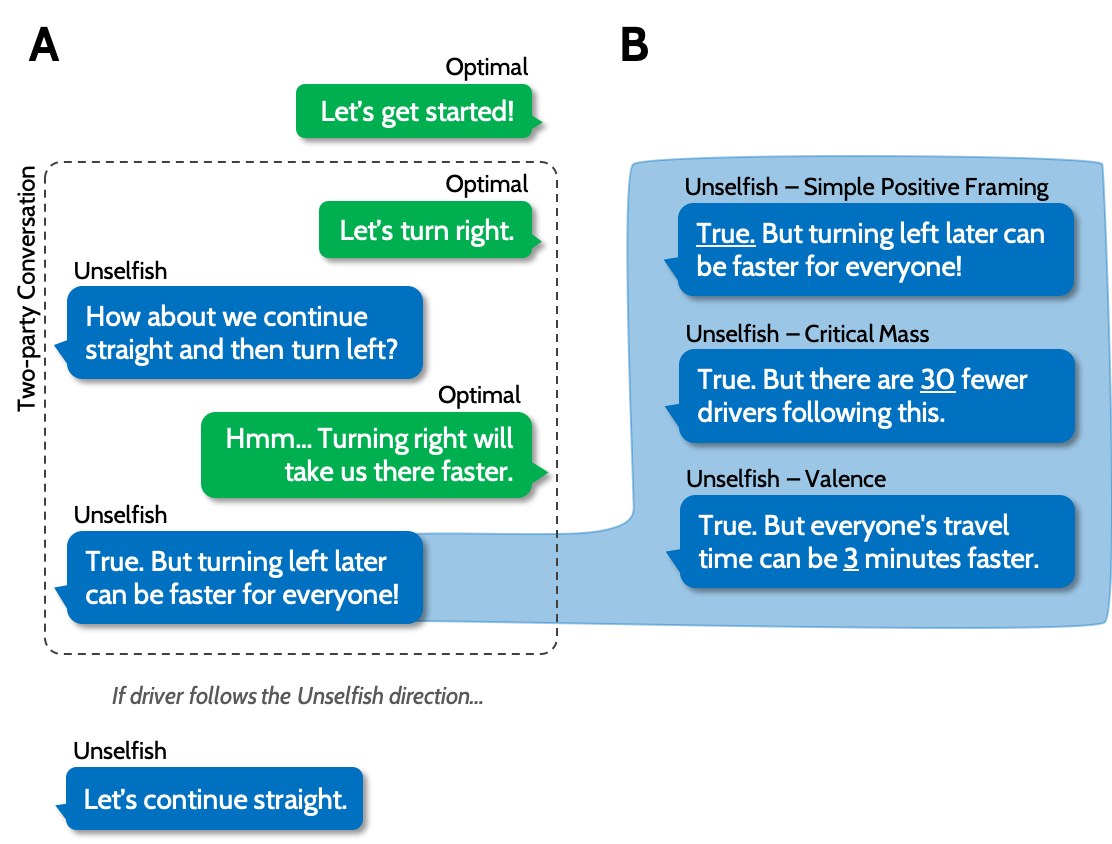
\includegraphics[scale=.75]{figures/s4-twopartyconvo.png}
  \caption{A) The sequence of voice guidance when a two-party conversation is played in the middle of following a route. B) The rationale spoken by the unselfish voice agent which differs depending on the motivative information of the personalized design version selected for a driver. The underlined items are different depending on the trip type. The values shown here are used during a home to work trip.}~\label{fig:s4-twopartyconvo}
\end{figure}

Conversations are only played as voice guidance when a driver chose the optimal route to follow. In this approach, the two-party conversation is a strategy to convince drivers to consider following an unselfish route for the rest of the trip. No conversations are played when the unselfish route is chosen at the beginning. To see all the voice guidance utterances for each route, please refer to Appendix \ref{AppendixC}.

\subsubsection{Voice Agents}
The Navigo approach will only use two voice agents. One will be a male voice and the other, a female voice. The default voice agent for delivering voice guidance will be the male voice. When a conversation is played, the female voice will say the recommended turn direction of an unselfish route. I opted to use distinctly different voices here because the evaluation of the original approach showed that some participants could not recognize that a conversation is already being played, especially when the two voice agents have the same gender. 

After the utterance of a two-party conversation, the voice guidance will be continued by the voice agent that uttered the selected turn direction. As an example, if the unselfish turn direction was followed, the voice guidance will be continued by the female voice agent. This gives the driver a sense of continuity and consistency, avoiding possible confusion. 

\subsubsection{Motivative Messages}
Instead of saying generic rationale during conversations, the female voice agent diversifies the rationale or second utterance based on the personalized motivative information. As an example, if the navigation application of a driver was personalized to use valence as motivative information, all the rationales spoken by the female voice agent in conversations will include the valence information. Table \ref{tab:s4-motivativemessages} shows the rationale that is spoken depending on the motivative information used.

\begin{table}[ht]
	\centering
	\caption{The different rationales spoken by the female voice agent that is based on the personalized motivative information.}
	\begin{tabular}{l l}
		\toprule
		\multicolumn{2}{l}{\textbf{Unselfish Route from Home to Work}} \\
		\midrule
		Framing & True. But turning left later can be faster for everyone! \\
		Critical Mass & True. But there are 30 fewer drivers following this. \\
		Valence & True. But everyone's travel time can be 3 minutes faster. \\
		\toprule
		\multicolumn{2}{l}{\textbf{Unselfish Route from Work to Home}} \\
		\midrule
		Framing & Hmm turning left on the next one can be faster for everyone! \\
		Critical Mass & Hmm there are 30 fewer drivers turning left on the next one. \\
		Valence & Hmm turning left on the next one can be 5 minutes faster \\
		& for everyone and you. \\
		\bottomrule
	\end{tabular}
	\label{tab:s4-motivativemessages}
\end{table}

When the unselfish route is chosen at the start, the motivative information shown in Table \ref{tab:s4-motivativeinfo} are spoken by the voice agent after a successful turn is made or when driving in a long road segment. 

\begin{table}[ht]
	\centering
	\caption{The spoken motivative information by the voice agent that is based on the personalization.}
	\begin{tabular}{l l}
		\toprule
		\multicolumn{2}{l}{\textbf{Unselfish Route from Home to Work}} \\
		\midrule
		Framing & Staying on this route makes it faster for everyone! \\
		Critical Mass & Only 30 drivers are taking this. \\
		Valence & Staying on this route can make everyone's travel time 3 minutes faster. \\
		\toprule
		\multicolumn{2}{l}{\textbf{Unselfish Route from Work to Home}} \\
		\midrule
		Framing & Staying on this route makes it faster for everyone! \\
		Critical Mass & Only 30 drivers are taking this. \\
		Valence & Staying on this route can make everyone's travel time 5 minutes faster. \\
		\bottomrule
	\end{tabular}
	\label{tab:s4-motivativeinfo}
\end{table}

\section{Related Works}
Navigo's concept builds upon previous works on diversification strategies, as well as personality-targeted design.

\subsection{Diversification Strategies}
Message and strategy diversification have been a cornerstone in many intelligent systems and web applications, especially in recommender systems and e-commerce websites. Typically, they would account for individual differences of users in deciding which message framing or recommendation to give. Other than using diversification strategies for commercial gain, several works have started investigating its use to promote behavior change in various contexts.

With a focus on behavior change, Kocielnik and Hsieh\cite{kocielnik2017send} used a positive motivational strategy to diversify the messages shown by an application to remind the performance of certain actions. They hypothesized that diversifying the messages based either on the action or the message recipient will avoid users from getting annoyed after seeing multiple messages. They found that messages that use concepts that are more familiar to the person were perceived as less annoying, thus supporting behavior change. In the context of incentives, Kocielnik and Hsieh\cite{hsieh2016you} based their diversification strategy on a person's values and motivations and evaluated whether this can encourage diverse participation from different types people. They found correlations between the self-reported human values and the rewards that they chose. Similar to the concept of Navigo, motivative information in displaying recommended routes and voice guidance will be diversified based on Self-Determination Theory's causality orientation and behavioral regulation type.

In terms of messaging, several works on promoting social activism and increased participation in online communities have used message diversification strategies with some success. To encourage increased participation of new users and one-time posts in online communities, McInnis et. al.\cite{mcinnis2016one} investigated the effect of diversifying call-to-action messages on the responsiveness of users to posts. For social activism, Savage et. al.\cite{savage2016botivist} developed Botivist which uses Twitter bots to identify and target users who has potential to enact activist causes. They used various message framings like evoking relatedness when reaching out to these identified users. However, the diversification was not so useful as the most direct call-to-action was found to be more effective in recruiting social activists. In the recent work of Grau et. al.\cite{grau2018personalized}, they explored personalizing motivation-supportive call-to-action messages to encourage students in a university to report community-related concerns on a crowd-civic platform. In a pairwise comparison of different call-to-action messages that is based on Self-Determination Theory, they found that there is no one message framing that will appeal to people with different types of motivation. Building on this insight, they built a design probe and investigated whether a personalization strategy will increase the number and length of reports submitted by volunteers. However, this was unsuccessful because they had issues in correctly identifying the type of motivation of their users. 

In this chapter, I also focus on diversifying messages delivered in voice guidance to encourage drivers to reconsider or stick to an unselfish route. Instead of using persuasion strategies, my goal is to use simple message framings based on Self-Determination Theory that will help drivers internalize their extrinsic motivation towards consistently choosing an unselfish route. 

\subsection{Personality-Targeted Design}
Personality-targeted design was first investigated by Nov and Arazy\cite{nov2013personality} when they showed how someone's level of conscientiousness can affect their level of engagement in a certain version of an interface. In gaming, a study showed that people prefer different gamification affordances based on their personalities. In a related study, Moon\cite{moon2002personalization} found that people are more likely to be receptive of the recommendation when the recommendation style matches their personality. Similarly in this work, I investigate how the different causality orientations and behavioral regulation types affect the selection of unselfish routes.

\section{Method}
In this section, I describe the methodology used for evaluating the feasibility of the Navigo approach. Because of the current mobility restrictions and the distancing requirements, all user studies were done online.

\subsection{Participants}
I recruited 10 participants from a convenience sample. As an inclusion criteria, they must be adults (18-60 y.o.) and have an active driver's license. They are composed of 7 males and 3 females, with ages that range from 25 to 47 years old. It was made sure that they are all new to the study and have not been part nor heard of the previous studies described in this thesis. They were not rewarded for participating in this study. 

In terms of driving years, 2 have only been driving for less than a year while 5 are driving for 1 to 5 years already. Only 3 participants have been driving for more than 5 years. In terms of driving experience based on total distance travelled, 3 participants have driven for less than 15,000km while 6 have driven for more than 25,000km already. All participants have used a navigation application while driving, with Google Maps and Waze as the popular tools. Two participants have been using them for less than year while 5 of them have been using theirs for 1 to 5 years already. Three (3) participants have been using their applications for 5 to 10 years. Most of them report that they often use navigation applications when they go on trips to a seldom visited or unknown location. Only 1 participant reported that they use it almost every time. When asked if they use voice guidance, only 4 participants answered Yes. 

\begin{figure}[t]
\centering
  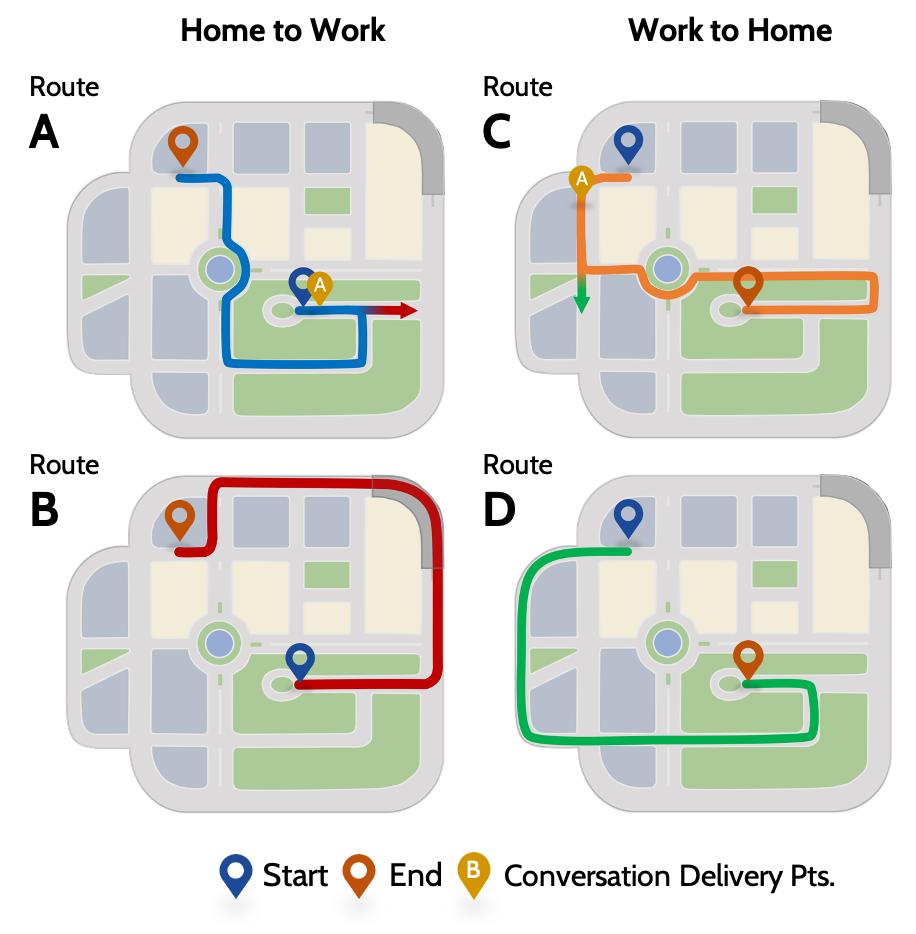
\includegraphics[scale=.7]{figures/s4-all-routes.png}
  \caption{The four routes used in the conduct of this user study. Route A and C are optimal routes while Routes B and D are unselfish routes. The route illustration for Routes A and C includes points on the map where the conversations were played. It also includes the turn direction that was suggested by the unselfish voice agent.}~\label{fig:s4-allroutes}
\end{figure}

\subsection{Setup \& Routes}
I used again the open-source CARLA simulator \cite{Dosovitskiy17} as our virtual driving environment. The Town3 map (Figure \ref{fig:s4-allroutes}) was selected because of its grid-like layout with many options for alternative routes. The map also features distinct land use areas and buildings that participants can easily distinguish (i.e. residential, commercial and industrial areas) for easy orientation in the environment. The virtual driving environment was used as is. For every participant session, we generate 60 random vehicles of different types around the map and they drive autonomously. 

% \begin{figure}[h]
% \centering
%   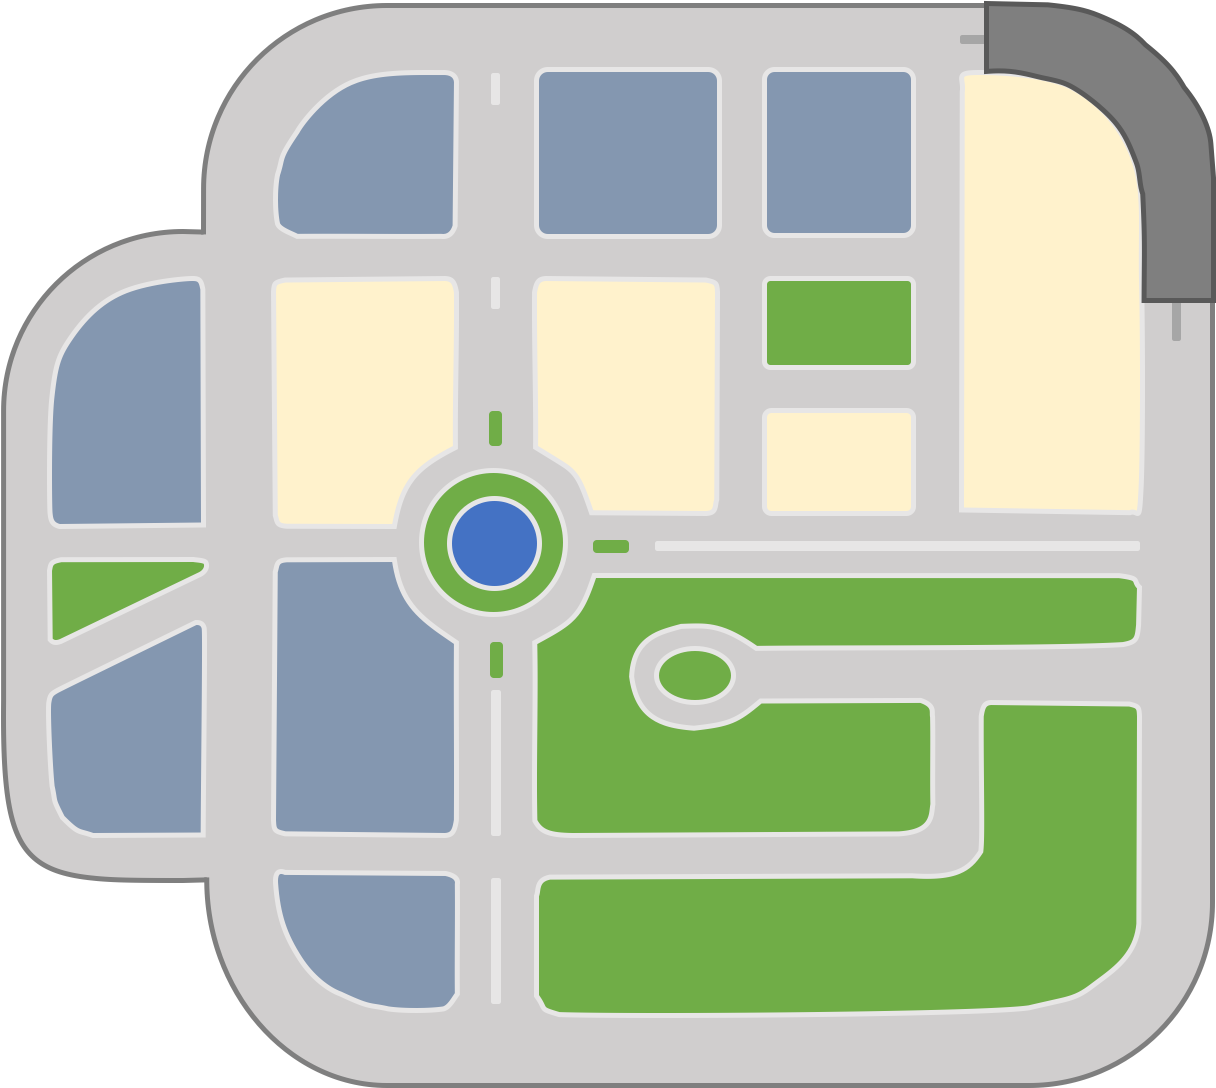
\includegraphics[scale=.3]{figures/s4-map.png}
%   \caption{The illustrated version of the CARLA Town3 map.}~\label{fig:s4-map}
% \end{figure}

I met the recruited participants and conduct the user study on Zoom. They were asked to use a headphone so that they can hear the voice guidance clearly. On my desktop that shares the screen, Figure \ref{fig:s4-setup} shows how the window of the virtual simulation and the prototype interface was laid out. The whole call was recorded with the participant's verbal consent.

\begin{figure}[h]
\centering
  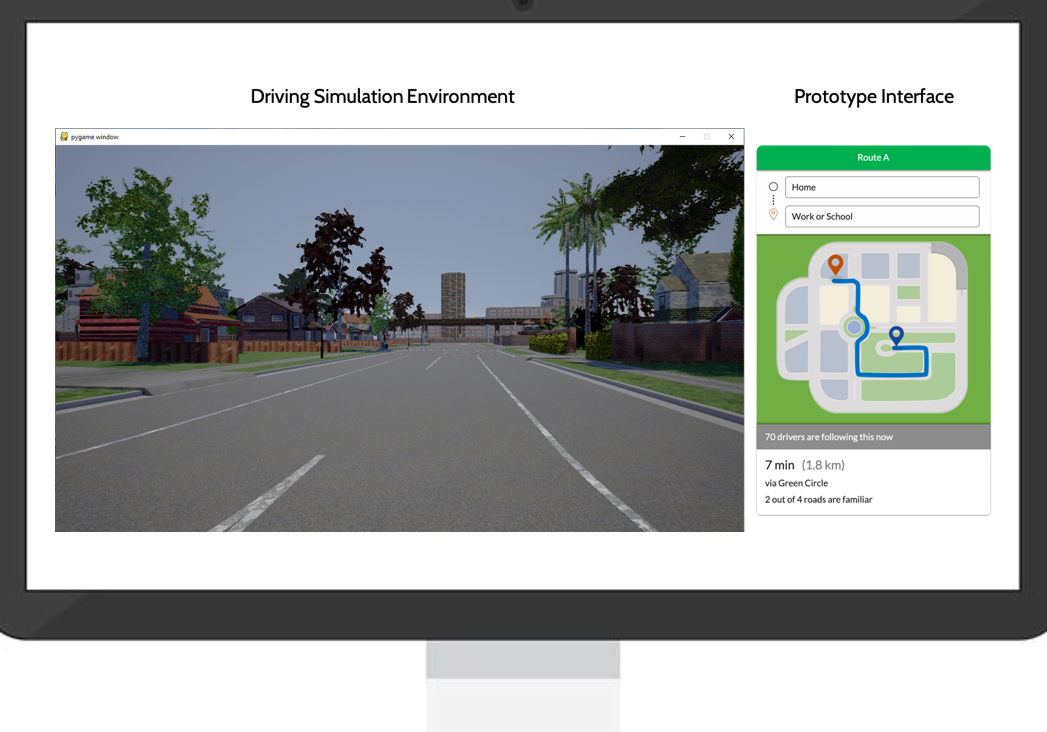
\includegraphics[scale=.45]{figures/s4-setup.png}
  \caption{The layout of the driving simulation window and the prototype interface during the driving task. THis is what the participants see while the experimenter is sharing the screen.}~\label{fig:s4-setup}
\end{figure}

For the purpose of this user study, I identified four (4) routes within the Town3 map, two (2) each for the Home-to-Work and Work-to-Home trips (Figure \ref{fig:s4-allroutes}). The optimal routes (Route A \& C) were chosen because they used quick and short turns, similar to shortcut paths. Both of them also use the roundabout because I wanted to lessen the number of traffic lights that the participants will encounter. The unselfish routes (Route B \& D) were more straightforward but required the participants to drive farther distances and with more traffic lights. I made sure that the optimal and unselfish routes are distinct, with little to no shared roads in their recommendations. 

\subsection{Conditions}
The goal of this user study is to find support to the key findings of the study described in Chapter \ref{ChapterPreTrip}. Specifically, I am curious how likely the participants will choose the unselfish route if they are shown a design version that is personalized to their causality orientation and or behavioral regulation styles. Thus, I designed this study to have 2 conditions. The first condition used the design version that was most preferred and significantly increased the likelihood of choosing an unselfish route. Participants in this condition are always shown thew combined use of simple positive framing and list of familiar roads. In the second condition, participants was shown personalized motivative and familiarity information. 

\begin{figure}[t]
\centering
  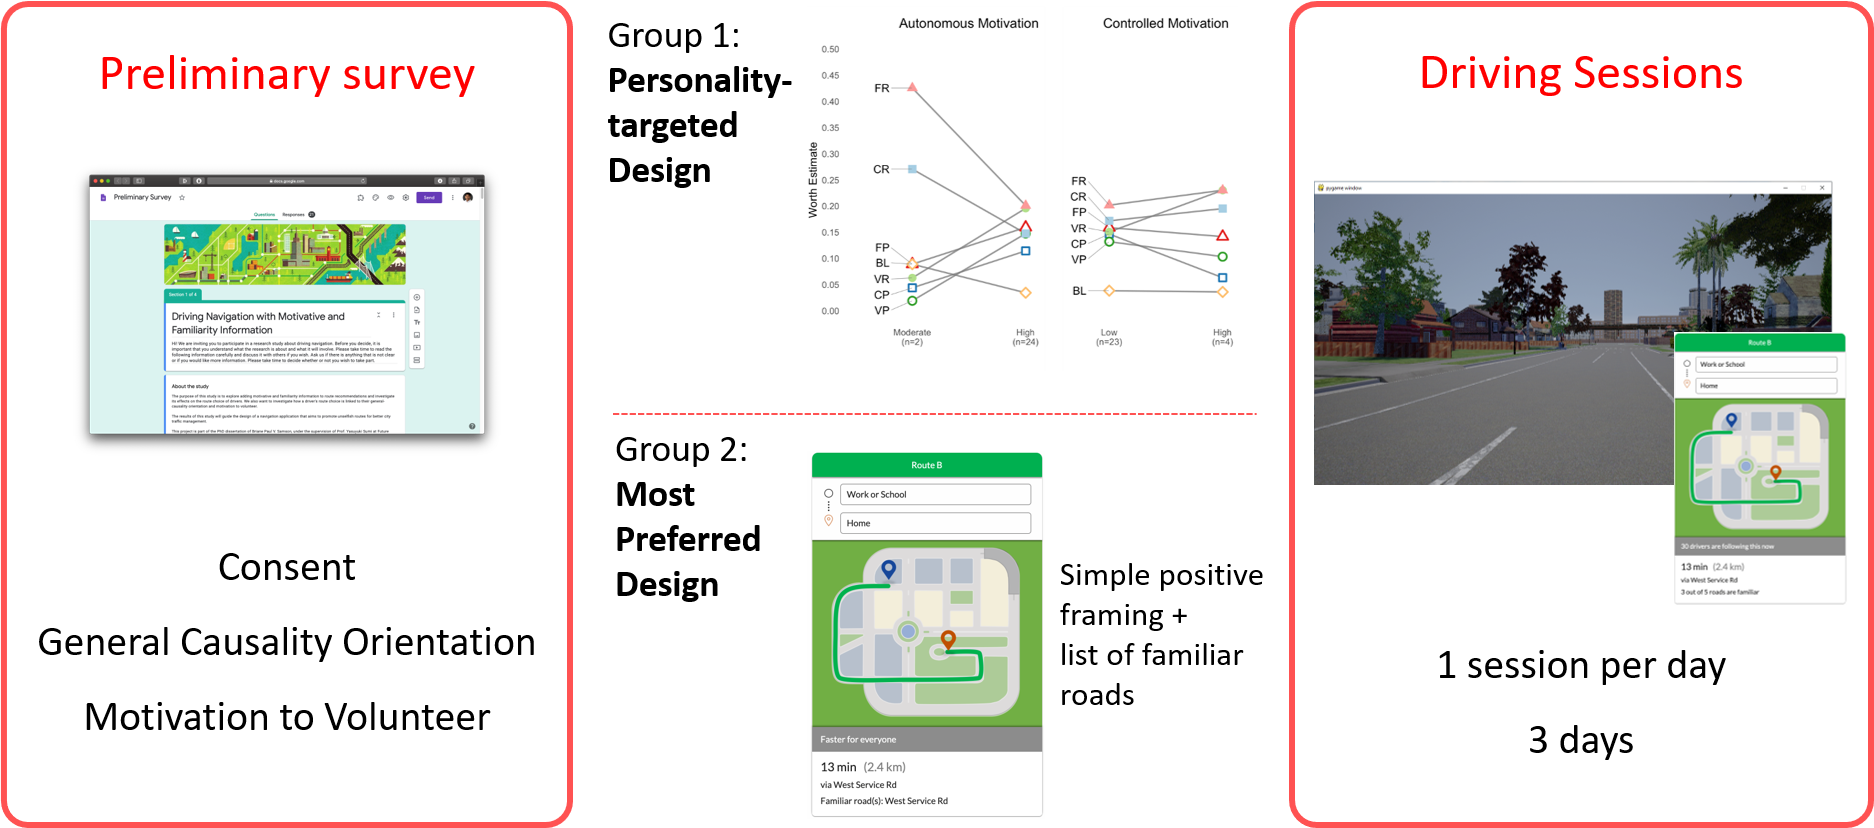
\includegraphics[scale=.45]{figures/s4-protocol.png}
  \caption{An overview of the study protocol. After the preliminary survey, participants were assigned randomly to two groups. After which, they were scheduled for driving sessions that spanned for 3 days. They were not always consecutive days.}~\label{fig:s4-protocol}
\end{figure}

\subsection{Protocol}
Before anything, participants were asked to answer a preliminary survey, which includes the consent form, questions that confirm they fit the inclusion criteria, the General Causality Orientation Survey, and the Motivation to Volunteer Survey. As shown in Figure \ref{fig:s4-protocol}, this is almost similar to the preliminary survey described in Chapter \ref{ChapterPreTrip}. Then, their causality orientation and behavioral regulation style scores were computed. These were used later to identify their personalized motivative and familiarity information. 

I conducted a between-subject Wizard of Oz study in which participants were asked to drive 2 times (Home-to-Work and Work-to-Home) in 3 separate sessions or Zoom calls. Participants were randomly assigned to 2 groups and were scheduled for the 3 sessions. In the first session, participants were given the baseline versions of the navigation application prototype (no motivative and familiarity information) and the voice guidance (no conversations and motivative information). The next 2 sessions were similar in which they were shown either a personalized motivative and familiarity information or the most preferred version. They also experienced the voice guidance with conversations and motivative information. 

At the beginning of the first session, I gave them an orientation about the goals of the research without giving away too much that would bias their performance. Then I asked if they would verbally consent to having the call recorded. All participants agreed and the tasks began.

Before they drive in the driving simulation environment, participants were asked to choose between 2 routes (Route A \& B). Based on their route choice, the voice guidance began uttering turn directions and the driving task began. Because the driving simulator experiment is done remotely, I was actually the one controlling the vehicle using keyboard commands. The participant was oriented to say what they want the vehicle to do. I did not move the vehicle in the simulation environment if I did not hear any command. I also stopped the vehicle at intersections and turning points to wait for the participant's next command. To keep things simple, participants were asked to just say ``turn left'' or just ``left'', ``go straight'' or ``follow this road'', and ``turn left'' or just ``left''. I and the participant did trial drives in the simulation environment to practice our coordination in controlling the vehicle. I was also constantly monitoring the video lag so that I can slow down the vehicle if the video rendering is late on their end. 

Each session begins with the task to drive from home to work. After they arrive at the destination, participants were given a short break then we continued with the return trip. For each trip, I took note of their pre-trip route choice and the turns they make after hearing a conversation or motivative information. These continued for 3 sessions and in the end, I asked them a few questions about their feedback on the information they saw when choosing a route, and their experience of hearing the voice guidance. 

\begin{table}[ht]
	\centering
	\caption{The general causality orientation and behavioral regulation style scores of the participants assigned to the personalization group. Unexpectedly, their personality-targeted design will use simple positive framing and show the list of roads (FR).}
	\begin{tabular}{l r r r r r r l}
		\toprule
		& \multicolumn{3}{c}{Causality Orientation} & \multicolumn{3}{c}{Behavioral Regulation} & Personality-Targeted\\
		& Raw & \% & Category & Raw & \% & Category & Version\\
		\midrule
		P1 & 6.75 & 0.96 & High & 4.25 & 0.85 & High & FR	\\ 
        P3 & 4.25 & 0.61 & Moderate & 4.25 & 0.85 & High & FR	\\ 
        P4 & 5.83 & 0.83 & High & 4.25 & 0.85 & High & FR	\\ 
        P5 & 3.50 & 0.50 & Moderate & 5.00 & 1.00 & High & FR	\\ 
        P8 & 5.92 & 0.85 & High & 4.00 & 0.80 & High & FR	\\ 
		\bottomrule
	\end{tabular}
	\label{tab:s4-personalization}
\end{table}

\section{Results}
In this section, I discuss the results of the route choice and driving navigation tasks. Further, I investigate how their route choices changed after each session and when they were shown additional motivative and familiarity information. I also discuss how often participants reconsidered their initial route choice after hearing two-party conversations in the voice guidance. 

\subsection{Personalization}
Because of the between-subject design, 5 participants were randomly assigned to the group which will experience personalized motivative and familiarity information. Despite being in the personalization group, all 5 participants were assigned the \textbf{FR} design version which is similar to the design version assigned by default to the other group (Table \ref{tab:s4-personalization}). 

\subsection{Making the Unselfish Choice}
In the first session, when there was no motivative and familiarity information shown to the participants, those with higher autonomy orientation already chose the unselfish route, Route B. There were already four (4) participants that chose the unselfish route in the H2W trip and two (2) in their W2H trips. P1 and P2 were consistent in choosing the unselfish route for both trips even with a baseline version. It should be noted that they have some of the higher autonomy orientation scores among participants. 

When presented with the motivative and familiarity information in the next sessions, Figure \ref{fig:s4-unselfish-result} shows that more participants made the unselfish choice. Consistent with the results in the previous study, drivers were more likely to choose Route B when the possible outcomes are presented. After using simple positive framing and showing the list of familiar roads in the 2nd session, 2 participants maintained their unselfish route choice while 3 participants shifted from following an optimal route to the unselfish route in their H2W trip. In the W2H trips, 7 participants chose the unselfish route. Two (2) participants were consistent with their first unselfish choice while 5 of them changed their mind to follow the unselfish route. 

In terms of trends, more and more participants choose Route B when driving from Home to Work, which supports the findings of my earlier study. However, in the Work to Home scenario, although there were also 6 participants who chose Route B, they were relatively less in the last session compared to the second session. Lastly, there were more participants who chose Route B in the last session.  

\begin{figure}[t]
\centering
  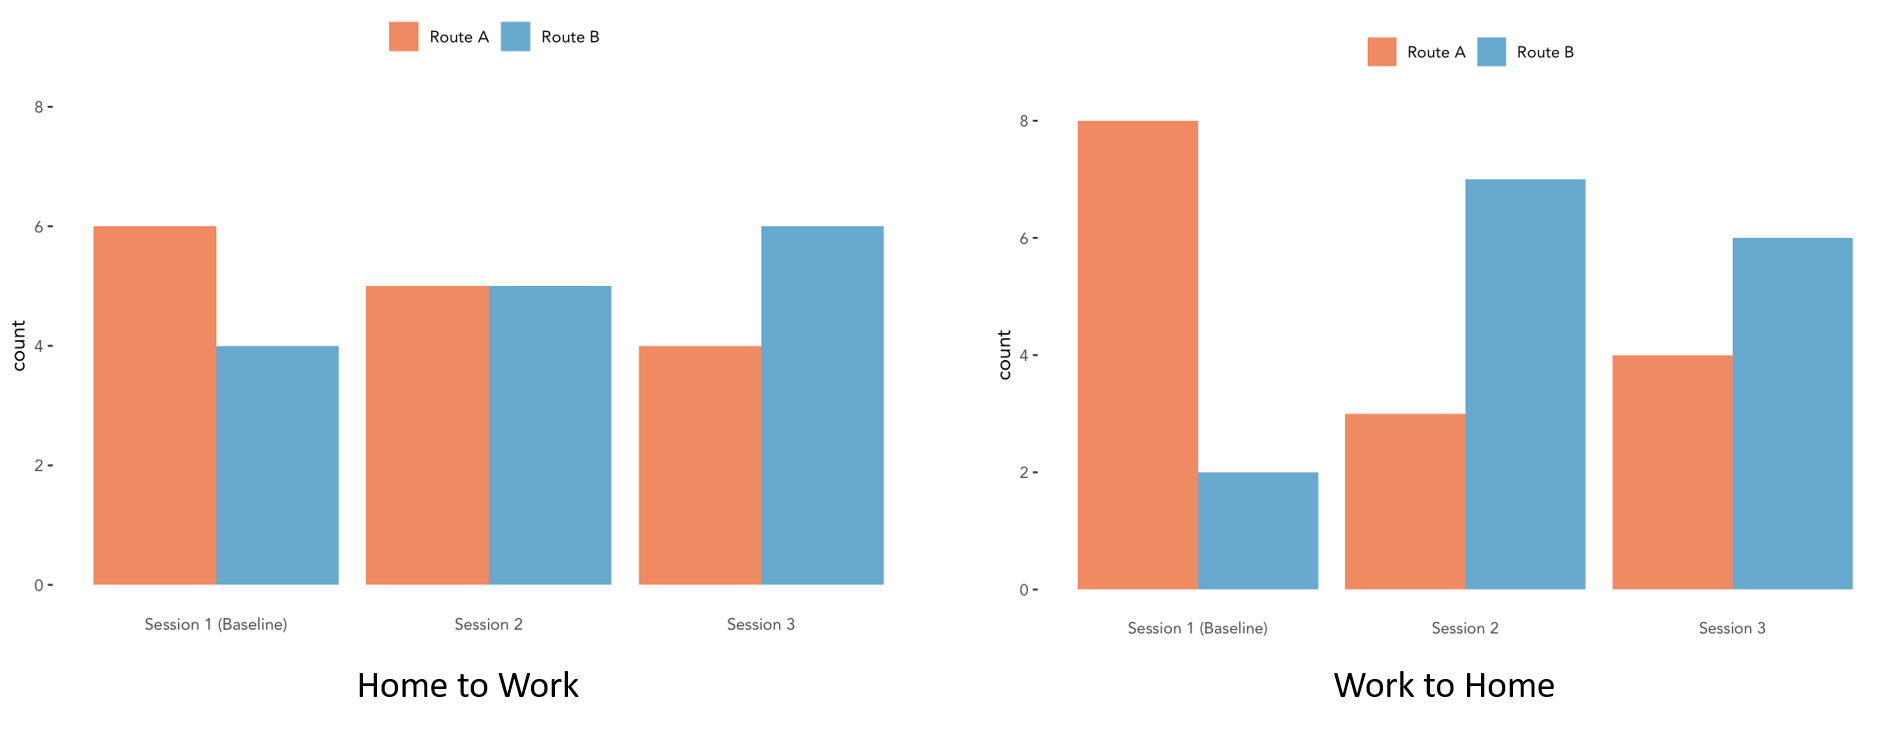
\includegraphics[scale=.45]{figures/s4-unselfish-result.png}
  \caption{\textbf{How effective is it in encouraging an unselfish choice after the first session?} This shows the number of times each route choice was selected by drivers in every session. The bar graph on the left shows the numbers for home to work trips, while the graph on the right shows the numbers for work to home trips.}~\label{fig:s4-unselfish-result}
\end{figure}

% \begin{table}[ht]
% 	\centering
% 	\caption{The patterns of route choice for the two type of trips in the study. Beside each pattern are the number of participants that manifested that route choice behavior.}
% 	\begin{tabular}{l r r}
% 		\toprule
% 		Route Choice Pattern & H2W & W2H \\
% 		\midrule
%             A A A & 3 & 2 \\
%             A B B & 3 & 3 \\
%             A B A & 0 & 2 \\
%             A A B & 0 & 1 \\
%             B A A & 1 & 0 \\
%             B A B & 1 & 0 \\
%             B B A & 0 & 0 \\
%             B B B & 2 & 2\\
% 		\bottomrule
% 	\end{tabular}
% 	\label{tab:s4-patterns}
% \end{table}

% \subsection{Choice Patterns}
% In this multiple session (longitudinal) study, the desired route choice patterns are BBB and ABB. These patterns mean that regardless of a participant's initial choice, they were able to change their mind and sustain their decision to follow an unselfish route in succeeding sessions. If at least 1 participant manifests any of these patterns, that is already indicative of the potential for encouraging behavior change by using simple positive framing combined with the list of familiar roads. Looking closely at Table \ref{tab:s4-patterns}, there were 3 participants that showed the ABB pattern in both H2W and W2H trips. For the BBB pattern, there were 2 participants each in the H2W and W2H trips. Half of the participants showed signs of sustained behavior change towards choosing unselfish routes in just 3 sessions. 

\begin{figure}[h]
\centering
  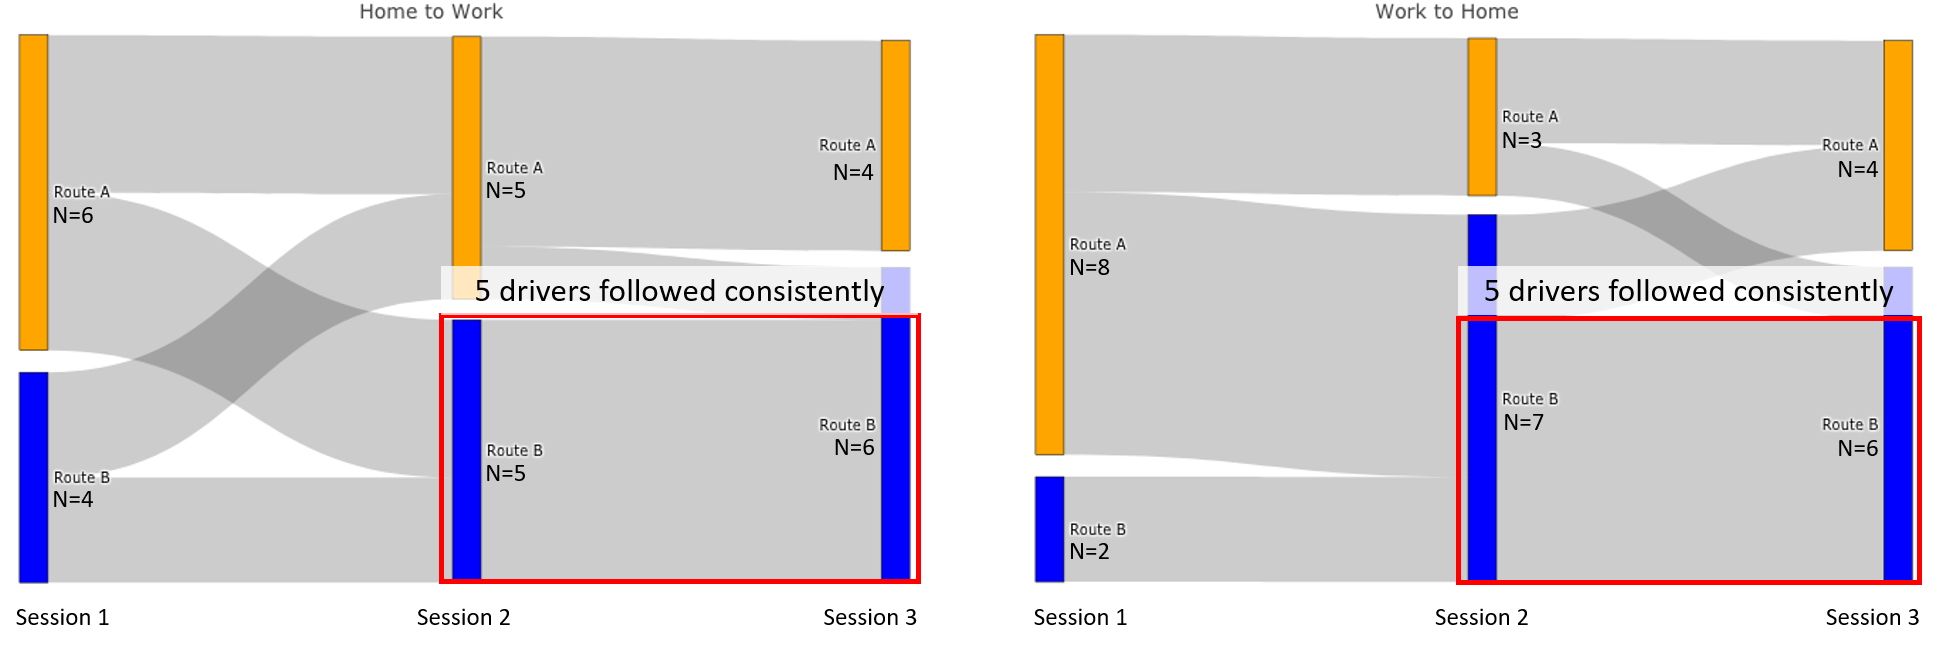
\includegraphics[scale=.45]{figures/s4-sustain-unselfish-results.png}
  \caption{\textbf{Can motivative and familiarity information help sustain the selection of an unselfish choice?} This shows the route choices of the 10 participants after each session. The flow from one session to the next indicates the switch in route choice. After following Route B in their second session, 5 participants continued to choose unselfishly in the third session.}~\label{fig:s4-sustain-unselfish-results}
\end{figure}

\subsection{Sustaining an Unselfish Choice}
Results also show evidence of how effective it is in encouraging the driver to continuously choose Route B. In Figure \ref{fig:s4-sustain-unselfish-results}, half of the participants (N=5) maintained their unselfish choice in both trip scenarios. The design of this study allowed us to see some evidence of sustained unselfishness unlike in the earlier one which only allowed one-shot decisions. Here, we were able to see how their decision-making change through repeated exposure to motivative and familiarity information. In the earlier study, a key finding was that most preferred combination was good in encouraging more drivers to follow the unselfish route but was not consistent in convincing individual drivers to continue choosing the unselfish route in different trip scenarios. Here, we found indicative evidence that this design version can make drivers continue following the unselfish route regardless of trip scenario. Based on the post-session interviews, another factor behind the sustained choice is that Route B was more straightforward compared to Route A. This is despite Route B being longer in terms of distance. 

\begin{figure}[h]
\centering
  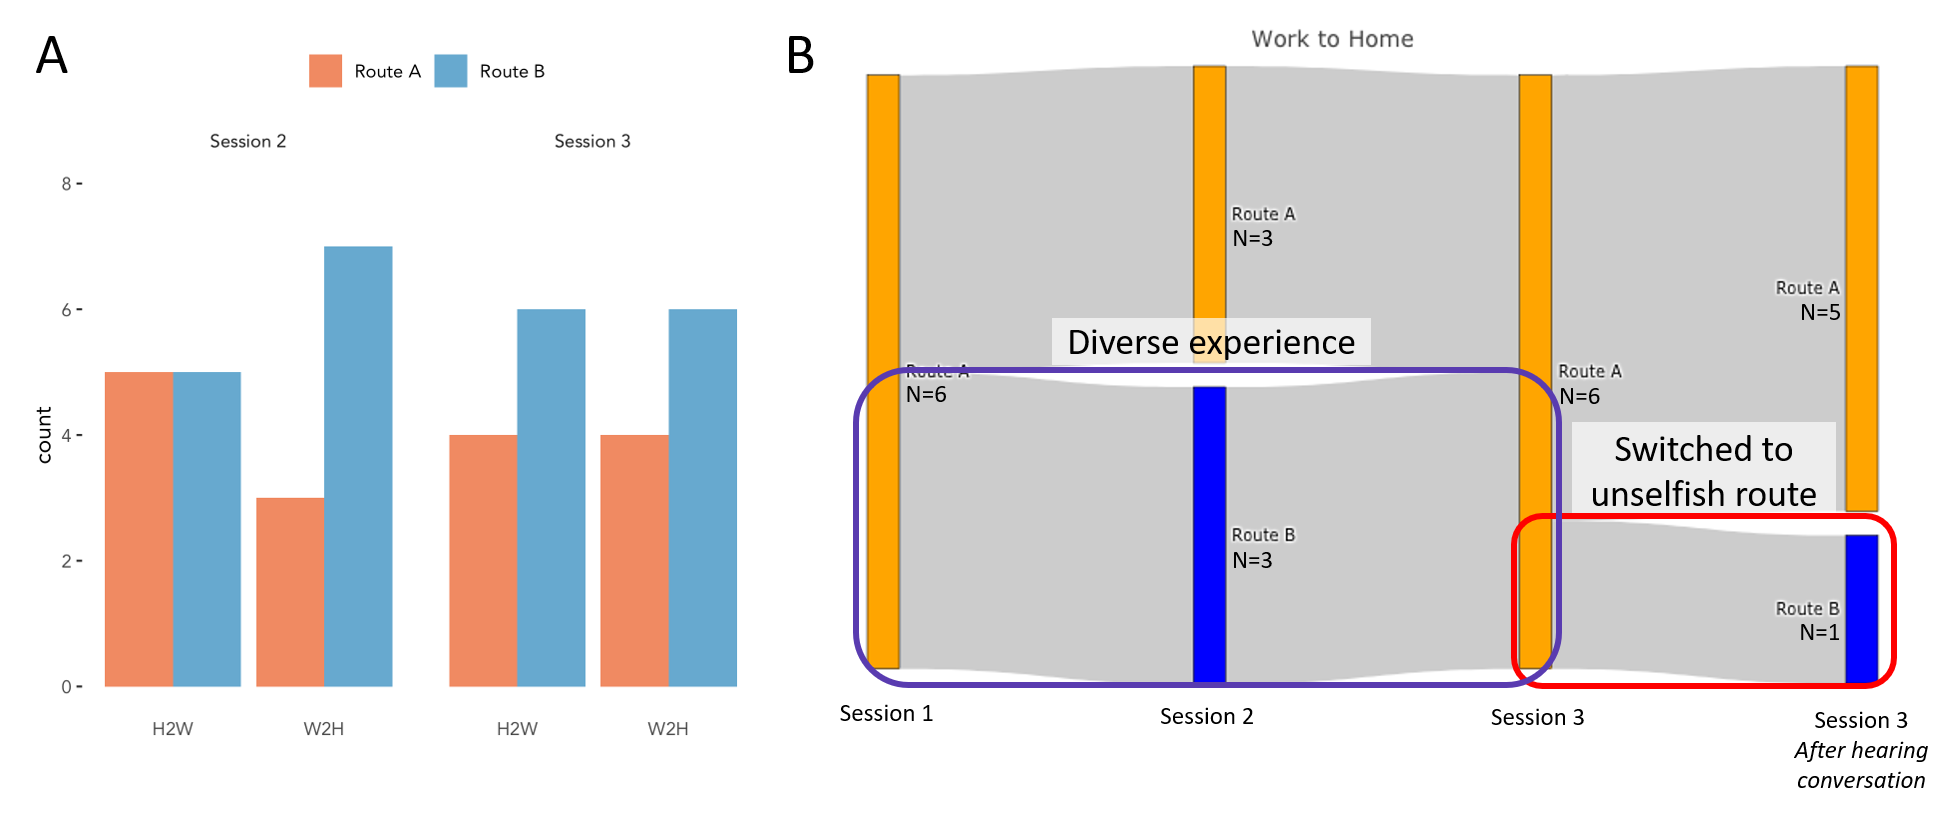
\includegraphics[scale=.45]{figures/s4-switch-unselfish.png}
  \caption{\textbf{Can two-party conversations convince drivers to switch to an unselfish route?} This shows the A) number of times the two routes were chosen in sessions 2 and 3, separated by the trip purpose. On the right are B) the different route choices made by 6 drivers who chose Route A in the third session.}~\label{fig:s4-switch-unselfish}
\end{figure}

\subsection{Switching to the Unselfish Route}
When the motivative and familiarity information were presented in sessions 2 \& 3, six participants still chose Route A over B for a total of 16 times -- 8 times in session 2 and 8 more times in session 3 (Figure \ref{fig:s4-switch-unselfish}A). In my approach, a two-party conversation is played as voice guidance to give alternative turn directions following the unselfish route. And a switch did happen in the last session of a participant when they were going home from work. 

Now, I will focus this analysis on the subset of participants who chose Route A when they were going home from work on the third and last session. Figure \ref{fig:s4-switch-unselfish}B shows the series of decisions made by 6 drivers. In their first and third sessions, all of them chose to follow the optimal route (Route A). The last column in Figure \ref{fig:s4-switch-unselfish}B shows the route that they continued to follow after hearing the conversation, and one of them switched to follow the unselfish route (Route B). When interviewed, they cited familiarity as reason for deviation. P10 answered that because they already tried both Route A and B, it was easier for them to assess the alternative unselfish route that was given in a conversation. In most cases, participants shared that they were rattled when they first heard the conversation between voice agents but as they got to hear it more in succeeding sessions, they were able to consider it more in their decision making. Indeed, this participant had a more diverse route choice before driving in session 3. Although this might seem like an outlier compared to those who did not make a switch at all, it should be noted that out of 6 participants who chose route A in the last session, only 3 of them had experience following both routes. This is indicative that diversity of previous choices and experiencing their outcomes can influence the effectiveness of the conversational technique. Another reason for the switch could be because participants feel less time pressure in the Work to home trip as shared in the interviews, which increases their tendency to explore. 

\begin{figure}[h]
\centering
  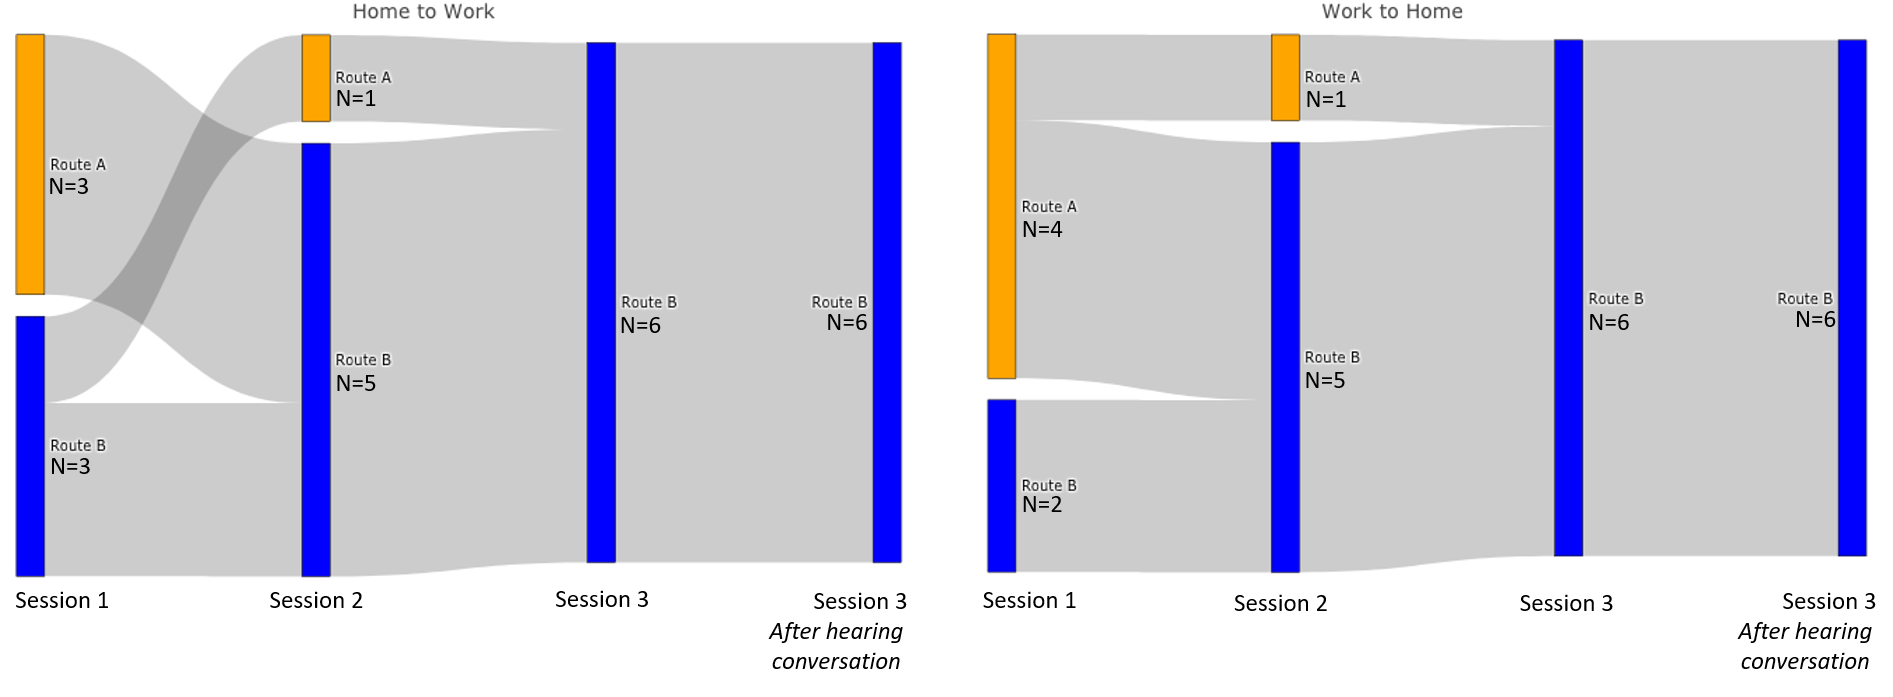
\includegraphics[scale=.45]{figures/s4-continue-follow-results.png}
  \caption{\textbf{Can two-party conversations encourage drivers to continue following an unselfish route?} The two figures show the route choices made by all participants in the home to work (left) and work to home (right) trips.}~\label{fig:s4-continue-follow-results}
\end{figure}

\subsection{Continuing an Unselfish Route}
When a participant selects the unselfish route, no conversations will be played. Instead, motivative information were spoken throughout the trip. When the motivative and familiarity information were presented in sessions 2 \& 3, eight participants decided to follow Route B for a total of 24 times -- 12 times in session 2 and 12 more times in session 3 (Figure \ref{fig:s4-switch-unselfish}A). In the Navigo approach, the voice agent utters motivative information that were like what was presented in the list of choices. Figure \ref{fig:s4-continue-follow-results} shows the series of decisions made by 4 drivers. Results show that the participants did not switch to the optimal route after choosing to follow the unselfish route. And even though 4 and 3 participants had diverse route choices before the last session, it did not seem to affect their decision to follow route B. Participants found it nice to hear the reassuring words of the voice agent and they agree with what was said. 
 
From the post-session interviews, participants shared that it was nice to hear the reassuring words of the voice agent and they agree with what was said. While it seems participants are positive with this approach, it is still hard to say whether these utterances actually encourage drivers to keep following the unselfish route. There are not much complex scenes in the driving simulator environment that could trigger changes in priority and behavior, except for stochastic traffic conditions. 

\section{Discussion \& Design Implications}
The results from this user study provided valuable insights on the value of providing a more holistic approach to encouraging better route choice and navigation. 

\subsection{Better Together}
In my earlier studies, I have identified specific design implications and a number of improvements that could improve the potential of each individual approach. Combining them in this study made it easier to realize those improvements. One major limitation of the original conversational approach was that the voice agents were trying to say too much information, even in critical turns. This led to higher subjective measures of workload and made it difficult to time when exactly they should be spoken. Since the pre-trip approach (Chapter \ref{ChapterPreTrip}) already provides familiarity information that the conversational approach also tries to provide, it was easier now to remove some information that made the voice agents verbose. Now in this holistic approach to motivating drivers to follow unselfish routes, it becomes more strategic and effective when we can use a number of media and modalities to deliver information and nudge our users.

\subsection{Motivative Voice Guidance}
Participants appreciated the motivative information spoken by the voice agent in the Navigo approach compared to my earlier approach. In the early work described in Chapter \ref{ChapterConversations}, the voice agent says the rationale behind the recommendation immediately after the turn suggestion. The timing and verbosity of that approach led some participants to ignore it in order to focus on making the navigational move. Here, the motivative information were spoken by the voice agent only when the driver is in a long stretch of road and not near or immediately turns. Another contributing factor could be the motivative information's positive and encouraging message (i.e. ``Staying on this route makes it faster for everyone!'').

\subsection{Diversification in Personalization}
In this approach, personalization was achieved by identifying one Self-Determination Theory construct or sub-scale that best represents a person (i.e. autonomy orientation, controlled motivation). However, that approach seems less personalized to some degree. If we inspect closely the causality orientation and behavioral regulation style sub-scales, it should be noted that the autonomy orientation and autonomous motivation scores are more likely to be higher compared to the other constructs. This means that the information strategy associated with consistently high constructs would always get used. One future exploration is the extension of my approach's personalization to consider all sub-scale scores. For example, if a driver has high autonomy and moderate controlled orientation, when should the navigation application personalize based on their high autonomy score and when to base it on their moderate controlled orientation? 

Our results in this chapter strongly supports the finding in Chapter \ref{ChapterPreTrip} that there is greater likelihood for a driver to choose an unselfish route when it is presented using simple positive framing and with a list of familiar roads. Thus it is safe to assume that most drivers would be convinced by its simplicity and explicitness. However, using the same messaging, despite being personalized, might start to seem boring, and reduce its positive utility and effect leading to annoyance and completely ignoring the message. Future exploration can learn from the work of Kocielnik and Hsieh\cite{kocielnik2017send} in implementing diversification strategies that connect more to the person than the task of driving itself. 

\section{Limitations}
The between-subjects design of the study was intended to see and compare the effect of using personalization in delivering motivative and familiarity information to the likelihood of choosing the unselfish route and its sustained selection. However, the biggest limitation of my convenient sample is that they did not have much diversity in general causality orientation and behavioral regulation styles. At the same time, even though I can achieve greater diversity, there also is not much personalization choices based on the results in Chapter \ref{ChapterPreTrip}. So far, there is only \textbf{FR}, \textbf{CR}, \textbf{VR} and \textbf{VP} design versions as options for personalization. 

Another big limitation is the driving simulation setup. While driving simulator experiments are believed to have better external validity\cite{fayyaz2020choices}, using it remotely might have confounding effects that we might not be aware of. 

\section{Conclusion}
In this chapter, I present Navigo, a holistic approach to encourage drivers to choose, follow, and stick to driving unselfish routes. Built on top of two previous approaches, I described various improvements based on their limitations. For example, I showed how the verbosity of the early conversational approach was reduced by off-loading the familiarity information on the list of choices. Then, I described how personalization can be achieved using causality orientation and behavioral regulation style scores, and how the voice guidance and two-party conversations were personalized. In a user study, I found supporting evidence that the use of simple positive framing combined with showing the list of familiar roads can encourage drivers to choose unselfish routes without explicit nudges. Their decisions were also sustained in succeeding trips after repeated use. Results also indicate the potential of personality-targeted two-party conversations in encouraging a driver to switch into following an unselfish route, although this would be more effective for someone with diverse route choice experiences. Lastly, the motivate messages uttered along the trip was appreciated by drivers and the lack of deviations indicate its potential in encouraging them to stick to flowing unselfish routes.
